\documentclass[../../../../main.tex]{subfiles}
\begin{document}

\begin{flushright}
\footnotesize\textit{【自動文字起こし・要確認】}
\end{flushright}

［解］(1)
\begin{align*}
f(x) &= \sqrt{2} a \pi x + c \cos \pi x + \sin \pi x \\
&= \sqrt{2} a t + c \cos t + \sin t \quad (t = \pi x) \equiv g(t)
\end{align*}
とすると
\[
g'(t) = \sqrt{2} a + c \cos t - \sin t
\]
だから $t_0$ の前後で $g'(t)$ の符号が変化するような $t_0$ の存在条件は，右図から

\begin{center}
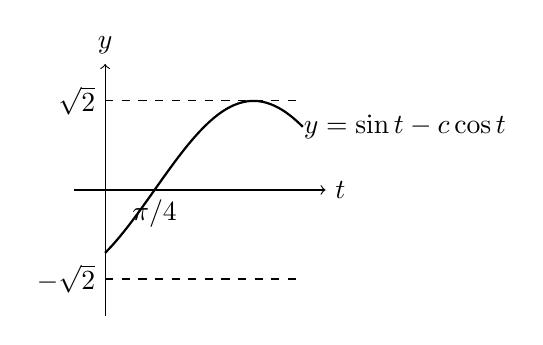
\begin{tikzpicture}[scale=0.8]
  \draw[->] (-0.5,0) -- (3.5,0) node[right] {$t$};
  \draw[->] (0,-2) -- (0,2) node[above] {$y$};
  \draw[domain=0:3.14, samples=50, smooth, thick] plot (\x, {1.414*sin(\x r - 0.785 r)});
  \draw[dashed] (0, 1.414) node[left] {$\sqrt{2}$} -- (3.14, 1.414);
  \draw[dashed] (0, -1.414) node[left] {$-\sqrt{2}$} -- (3.14, -1.414);
  \node[below] at (0.785, 0) {$\pi/4$};
  \node[right] at (3, 1) {$y = \sin t - c \cos t$};
\end{tikzpicture}
\end{center}

\[
-\sqrt{2} < \sqrt{2} a < \sqrt{2}
\]
\[
\therefore 0 < a < 1 \quad (\because a > 0)
\]

(2)

\begin{center}
\begin{tikzpicture}[scale=0.8]
  \draw[->] (-0.5,0) -- (4.5,0) node[right] {$t$};
  \draw[->] (0,-1.5) -- (0,2.5) node[above] {$g'(t)$};
  \draw[domain=0:4, samples=50, smooth, thick] plot (\x, {cos(\x r * 1.5) + 0.8});
  \draw[dashed] (0, 1.8) node[left] {$\sqrt{2}a + 1$} -- (4, 1.8);
  \draw[dashed] (0, 0.8) node[left] {$\sqrt{2}a$} -- (4, 0.8);
  \draw[dashed] (0, -0.2) node[left] {$\sqrt{2}(a-1)$} -- (4, -0.2);
  \fill (1.05, 0) circle (2pt);
  \fill (3.14, 0) circle (2pt);
  \node at (2, -1) {（オブラス）};
\end{tikzpicture}
\end{center}

$g'(t)$ が周期 $2\pi$ の周期関数であることから，$0 \le t < 2\pi$ で $g'(t)$ の符号が $t_0$ の前後で正から負になるような $t_0$ があって，$t = t_0 + 2n\pi \, (n \in \mathbb{Z})$ においては $g(t)$ は極大になる。

従って，極大となる点の座標を $(X, Y)$ とすると $t = \pi x$ から
\[
X = \frac{t_0}{\pi} + 2n, \quad Y = \sqrt{2} a \left( \frac{t_0}{\pi} + 2n \right) + c \cos t_0 + \sin t_0
\]
従って，たしかに $(X, Y)$ は直線上にあり（$n$ を消せばわかる），その $X$ 座標の間隔が $2$ だから，等間隔である。

\newpage

\end{document}
